\documentclass[10pt,a4paper]{article}
\usepackage{amsmath}
\usepackage{amsfonts}
\usepackage{amssymb}
\usepackage{natbib}
\usepackage{graphicx}
\usepackage[left=2cm,right=2cm,top=2cm,bottom=2cm]{geometry}
\usepackage{arydshln}

\title{Unbiased Noise Characterization for Geodetic Data}
\author{Trever T. Hines and Eric A. Hetland}
\begin{document}

\maketitle
\section{Introduction}\label{sec:Introduction}


The noise in geodetic data, which we consider to be any observed deformation that is not representative of the cohesive crustal block, is temporally correlated. It is necessary to accurately quantify this noise before the data is used to make geophysical inferences. A power-law relationship is often used to described the frequency content of noise in geodetic data \citep{Agnew1992}.  The power spectral density of power-law noise is described as 

\begin{equation}\label{eq.PowerLaw}
  P(f) = P_o f^{-n}
\end{equation}
where $f$ is frequency, $n$ is the spectral index and $P_o$ is the amplitude. Analysis of time series from strain and tilt meters \citep{Wyatt1982,Wyatt1989}, electronic distance measurements \citep{Langbein1997}, and short-baseline GPS \citep{King2009} indicates that temporally correlated noise can be attributed, at least in part, to an unstable geodetic monument. The referenced studies have found that localized motions of the monument can be modeled as a random walk process ($n=2$). Global or regional GPS data, which is prone to additional non-physical sources of error \citep[e.g.][]{King2010}, has been described as a combination of white noise ($n=0$) and flicker noise ($n=1$) \citep{Zhang1997,Mao1999,Williams2004}. \citet{Langbein2008}, who used longer GPS timeseries,  found that GPS data in Southern California and Nevada contains white noise and some combination of flicker noise and random walk noise that varies between stations. It was suggested by \citet{Langbein2008} that random walk noise in GPS data can be attributed to monument instability while flicker noise can be attributed to non-physical errors introduced in deriving the displacement timeseries.  

No single noise model is universally appropriate for geodetic data, and the most rigorous of studies involving geodetic data should estimate a noise model for each station.  \citet{Langbein1997} introduce a maximum likelihood (ML) method for determining the optimal values for $P_o$ and $n$ (or the hyperparameters for any other assumed model). This method has become the standard technique for characterizing noise in geodetic data \citep{Langbein2004,Langbein2008,Zhang1997,Mao1999,Williams2004,King2009,Murray2017}.  

Recently, \citet{Langbein2012} demonstrated with synthetic data consisting of white and colored noise that the ML method is biased towards inferring a small component of colored noise in short timeseries.  The bias is appreciable when the length of the timeseries is less than or comparable to the cross-over period, which is the period at which the power of the colored noise exceeds the power of the white noise. \citet{Langbein2012} claims that the colored noise tends to be underestimated because it is indistinguishable in the power spectra of the data. We do not find this explanation to be satisfying. If the length of the timeseries is comparable to or less than the cross-over period then we would expect the estimated colored noise to have a high variance but this does not explain why there is a bias. In this paper we explain why the ML method from \citet{Langbein1997} is biased, and we provide a correction to the ML method which removes the bias without adding any significant computational burden. 

\section{Maximum likelihood methods}

Let $\mathbf{d_*}$ denote a column vector of $n$ observations made at times $\{t_1,t_2,\dots,t_n\}$. We treat $\mathbf{d_*}$ as a realization of the random vector

\begin{equation}\label{LangbeinModel}
  \mathbf{d} = \mathbf{Gm} + \mathbf{\epsilon},
\end{equation}
where $\mathbf{\epsilon}$ is the data noise vector, $\mathbf{G}$ is a $n \times m$ matrix with linearly independent columns that are used to describe geophysical signal in $\mathbf{d}$ (e.g. secular rates, coseismic offsets, postseismic transience, etc.), and $\mathbf{m}$ is a column vector of $m$ model parameters which have uninformative priors (i.e. $\mathbf{m} \sim \mathcal{N}(\mathbf{0},\lambda\mathbf{I})$ in the limit as $\lambda \to \infty$).  We assume that the data noise can be described as $\mathbf{\epsilon} \sim \mathcal{N}(\mathbf{0},\mathbf{\Sigma}(\mathbf{\theta}))$, where $\mathbf{\theta}$ are the hyperparameters which we want to find appropriate values for. Ideally, we would selects $\mathbf{\theta}$ such that the probability of drawing $\mathbf{d_*}$ from $\mathbf{d}$, $p_\mathbf{d}(\mathbf{d_*}|\mathbf{\theta})$, is maximized. However, the uninformed prior on $\mathbf{m}$ makes $\mathbf{d}$ improper and $p_\mathbf{d}$ is zero for all choices of $\mathbf{\theta}$. We must instead seek an alternative likelihood function to maximize. 

The ML method from \citet{Langbein1997} chooses $\mathbf{\theta}$ such that the probability of sampling the least squares residual vector,

\begin{equation}\label{ResidualRealization}
  \mathbf{r}_* =  \left(\mathbf{I} - \mathbf{G}\left(\mathbf{G}^T\mathbf{\Sigma}^{-1}\mathbf{G}\right)^{-1}\mathbf{G}^T\mathbf{\Sigma}^{-1}\right)\mathbf{d_*},
\end{equation}  
from $\mathbf{\epsilon}$ is maximized. To put it explicitly, The ML method maximizes the probability density function

\begin{equation}\label{MLProb}
p_\mathbf{\epsilon}(\mathbf{r}_*|\mathbf{\theta}) = 
\left(\frac{1}{(2\pi)^n\left| \mathbf{\Sigma}(\mathbf{\theta}) \right|}\right)^{\frac{1}{2}} 
e^{-\tfrac{1}{2}\mathbf{d}_*^T\mathbf{K(\mathbf{\theta}})\mathbf{d}_*}
\end{equation}
with respect to $\mathbf{\theta}$, where
\begin{equation}
\mathbf{K} = \mathbf{\Sigma}(\mathbf{\theta})^{-1} - 
             \mathbf{\Sigma}(\mathbf{\theta})^{-1}\mathbf{G}
             \left(\mathbf{G}^T\mathbf{\Sigma}(\mathbf{\theta})^{-1}\mathbf{G}\right)^{-1}
             \mathbf{G}^T\mathbf{\Sigma}(\mathbf{\theta})^{-1}.
\end{equation}
The ML method implicitly assumes that $\mathbf{r}_*$ is a representative sample of $\mathbf{\epsilon}$. This assumption is only valid when $n$ is sufficiently large. To elaborate, we note that $\mathbf{r_*}$ is a sample of the random variable

\begin{equation}\label{ResidualVariable}
  \mathbf{r} =  \left(\mathbf{I} - \mathbf{G}\left(\mathbf{G}^T\mathbf{\Sigma}^{-1}\mathbf{G}\right)^{-1}\mathbf{G}^T\mathbf{\Sigma}^{-1}\right)\mathbf{d},
\end{equation}  
which is distributed as
\begin{equation}\label{ResidualDistribution}
  \mathbf{r} \sim \mathcal{N}\left(\mathbf{0},\mathbf{\Sigma} - \mathbf{G}\left(\mathbf{G}^T\mathbf{\Sigma}^{-1}\mathbf{G}\right)^{-1}\mathbf{G}^T\right).
\end{equation}
The term being subtracted in eq. (\ref{ResidualDistribution}) is the covariance of the least squares prediction vector, which will typically get smaller as $n$ increases. The distribution of $\mathbf{r}$ will then tend towards that of $\mathbf{\epsilon}$ as $n$ increases. Thus we can only assume that $\mathbf{r}_*$ is a representative sample of $\mathbf{\epsilon}$ when $n$ is sufficiently large. We can also observe from eq. (\ref{ResidualDistribution}) that the variance of $\mathbf{r}$ will always be less than the variance of $\mathbf{\epsilon}$.  We believe this is the reason why the ML method from \citet{Langbein1997} is biased towards underestimating the noise in short timeseries.

Having demonstrated that the ML method from \citet{Langbein1997} is biased, we move on to discuss the restricted maximum likelihood (REML) method for selecting $\mathbf{\theta}$.  The REML method was introduced by \citet{Patterson1971} and is now accepted in the Kriging literature as an unbiased method for estimating covariance functions \citep[e.g.][]{Cressie1992}. The REML method can be understood by first considering a $(n-m)\times n$ matrix $\mathbf{R}$ which has the properties $\mathbf{R}\mathbf{R}^T = \mathbf{I}$ and $\mathbf{R}\mathbf{G}=\mathbf{0}$.  We then consider the random variable $\mathbf{x}=\mathbf{R}\mathbf{d}$, which can be interpreted as the projection of $\mathbf{d}$ onto a subspace that is orthogonal to the columns of $\mathbf{G}$. As opposed to $\mathbf{d}$, $\mathbf{x}$ is a proper random variable since it is independent of the prior on $\mathbf{m}$. The REML method chooses $\mathbf{\theta}$ such that the probability of drawing $\mathbf{x}_*=\mathbf{R}\mathbf{d}_*$ from $\mathbf{x}$, $p_\mathbf{x}(\mathbf{x}_*|\mathbf{\theta})$, is maximized. As noted by \citet{Harville1974}, the particular choice for $\mathbf{R}$ does not matter because it will only change the likelihood function which we are maximizing by a scale factor. Following \citet{Harville1974}, we then conveniently choose $\mathbf{R}$ to satisfy $\mathbf{R}^T\mathbf{R} = \mathbf{I} - \mathbf{G}(\mathbf{G}^T\mathbf{G})^{-1}\mathbf{G}^T$.  The probability density function for $\mathbf{x}$ can then be written as 

\begin{equation}\label{REMLProb}
p_\mathbf{x}(\mathbf{x}_*|\mathbf{\theta}) =
\left(\frac{\left|\mathbf{G}^T\mathbf{G}\right|}
           {(2\pi)^{n-m}
            \left| \mathbf{\Sigma}(\mathbf{\theta}) \right| 
            \left| \mathbf{G}^T\mathbf{\Sigma}(\mathbf{\theta})^{-1}\mathbf{G} \right|}\right)^{\frac{1}{2}} 
e^{-\tfrac{1}{2}\mathbf{d}_*^T\mathbf{K}(\mathbf{\theta})\mathbf{d}_*} .
\end{equation}

Note the similarity between eq. (\ref{REMLProb}) and eq. (\ref{MLProb}). If programmed efficiently (see Appendix A) and if $m \ll n$, the computational cost of the REML method is practically equivalent to that of the ML method from \citet{Langbein1997}. What remains to be determined is whether the REML method remediates the bias in the ML method. We demonstrate that this is indeed the case with a numerical test. 

\section{Synthetic demonstration}
We compare the REML method and the ML method from \citet{Langbein1997} by using the two methods to estimate the hyperparameters from snythetic data. This demonstration is modeled after the demonstration from \citet{Langbein2012} which highlights bias in the ML method. Our synthetic noise is a combination of white and random walk noise, which has a power spectral density described by

\begin{equation}\label{SyntheticFreq}
P(f) = \frac{\sigma_{rw}^2}{2\pi^2 f^2} + 2\sigma_w^2\Delta t,
\end{equation}  
where $\sigma_{rw}$ and $\sigma_w$ are hyperparameters for the random walk and white noise components, respectively. $\Delta t$ is the sampling period, which is set at one day. The cross-over frequency for the synthetic noise noise is then
\begin{equation}\label{Crossover}
f_o = \frac{1}{2\pi\sqrt{\Delta t}}\frac{\sigma_{rw}}{\sigma_w}.  
\end{equation}
In order to use the ML or REML method, we must express the power-law relationship in the frequency domain as a covariance matrix in the time domain. A general procedure for doing  so can be found in \citet{Langbein2004}. The components of the covariance matrix corresponding to eq. (\ref{SyntheticFreq}) can be concisely written as

\begin{equation}\label{Covariance}
\Sigma_{ij} = \sigma_{rw}^2 \min(i\Delta t,j\Delta t) + \sigma_w^2 \delta_{ij},
\end{equation} 
where $\delta_{ij}$ is the Kronecker delta function. Similar to \citet{Langbein2012}, we set $\sigma_{rw} = 1.3$ mm/yr$^{0.5}$ and $\sigma_w = 1.1$ mm. We generate 10,000 synthetic noise timeseries, which each have a length of 2.5 yr. 

We consider $\sigma_w$ to be known, for the sake of simplicity, and we just want to estimate $\sigma_{rw}$ from the synthetic data. While our synthetic data just consists of noise, we assume that the unknown underlying geophysical signal (i.e. $\mathbf{G}\mathbf{m}$) consists of a constant and linear trend. We estimates $\sigma_{rw}$ with the ML and REML methods using varying lengths of the synthetic timeseries. The timeseries lengths range from 0.1 yr to 2.5 yr at 0.1 yr increments. The distribution of estimated $\sigma_{rw}$ is shown in Figure \ref{fig:EstimateRW}.     

\begin{figure}
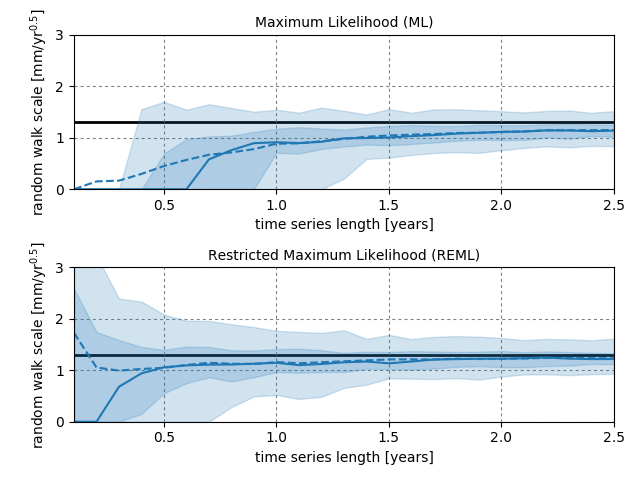
\includegraphics[scale=1.0]{figure_1.png}
\caption{Comparison of ML and REML method over varying lengths of the synthetic timeseries. The black line indicates the true random walk scale ($\sigma_{rw}=1.3$), the light blue region shows the 10-90 percentile of estimates, the dark blue region shows the 30-70 percentile of estimates, the solid blue line indicates the median, and the dashed blue line indicates the mean. Note that $f_o^{-1} \approx 0.3$.}   
\label{fig:EstimateRW}
\end{figure}



We use the ML and REML methods to estimate $\sigma_{rw}$, and we vary the portion of the .    
considered known, we assume that the white noise component We then use the ML method and the REML method to estimate   

  

, which corresponds to $f_o^{-1} \approx 0.3$ yr.

We compare the two  remains to be determined is whether the REML metho


We disagree with the heuristic that the length of the timeseries sould be ~5 times larger than the cutoff period.

virtually equivalent to for will both equations can be evaluated with essentially equivalent computation cost. valuating the two expressions use 
In order to make this problem tractible, we assume some functional form for $\mathbf{\Sigma}$. For example, if we assume that $\mathbf{\epsilon}$ is Brownian motion then the components of $\mathbf{\Sigma}$ can be written as

\begin{equation}\label{RandomWalk}
  \Sigma_{ij} = \sigma^2\min(t_i,t_j).
\end{equation}

Not

With this assumption we have converted to 
which converts the intractible problem of optimizing $\mathbf{C_d}$ into a more tractible problem of optimizing the hyperparameter $\sigma$. 

can be described  components of the covariance matrix can be   if the $\mathbf{d_*}$ was observed at times $\mathbf{t} = {t_1,t2,...,t_n}$, then we can      

The MLE method, 

  f the data which we do not consider to be noise ( which     and its covariance, $Cd$, is what we want to estimate.  

In fact, the bias in the MLE method is well recognized in the Kriging literature \citep[e.g][]{Cressie1992} and the correction that we propose has been known of since the work of \citet{Patterson1971}. Nonetheless, we find         

In this paper we an alternate explanation for the bias in the MLE method and we also     

be high variance in estimated colored noise should have a high variance but not a bias.   and we reasoning can how find this to be a satisfactory explanation for the bais

This is not a satisfying explanation bsatisfactory explanation for the bias, since it only explains why we would expect a high variance in estimated colored noise components.

Rather, this rationale would suggest that estimated components of colored noise would have a high variance not not biased. in 

rather we find it as an explanation    

the power spectral density is dominated by white noise and there will be little evidence for a colored noise component.   \citet{Langbein2012} reasoned that this bias can be noise power spectral density for such a short timeseries is dominated by the white noise, making the colored noise component indistinguishable.  We do not find this explanation to be satifactory. If the absense of evidence for colored noise does not ,  explains why there should be a high variance in the  estimating a smla   

   

would be dominate by the white component  masked by the white component   

The rational being that the frequency content of any colored noise is    white noise power and colored noise 

the time series istowards inferring  baised  the esimates to  showed the MLE method tends to estimate an     
 for used many studies on noise analysis    


  rigorous studies on geodetic  it should be common practice to estimate and optimal noise model.  no clear model which 

In To determine which noise model is most appropriate,     

in  who used longer GPS time series.  \citet{Langbein2008} showed that the amplitude of the power law noise and its spectral index can vary depending on the station location and the how the station was installed. Thus a rigorous study involving geodetic data would require that a noise model be determined for each station.  would    the most rigorous      

The most common approach to techniques for determinng  


There is not a generally accepted noise model for geodetic data, and the most rigorous geodetic analysis would require estimating a noise model for each geodetic time series.  

    ,  other tmodeling assumptions made in deriving the displacement time ich can have non-physical sources of error related to modeling assumptions in deriving the d,  be contanimated sources of errors  related to the GPS system,            Studies of geodetic mon  


can be derived from the geodetic data can be overly confident \citep[e.g][]{Mao1999}.  can be unduly cbiased  is necessary to accurately quantify this noise using the data to make geophysical inferences 


This can be attributed to localized motion of the geodetic monument \citep[e.g.][]{Wyatt1982,Wyatt1989,Agnew1992,King2009}. For GPS data, there are several assumptions and models involved  \citet{Langbeing2008,Langbein2012} has suggested that non-physical, temporally correlated noise could be introduced by errors in deriving the displacement time series.  

It is generally accepted that the frequency content of this noise can be accurately described with a power law relationship.  There is no generally accepted spectral index, since that can vary depending on the location and the type of instrument being used.  For example, short baseline instruments such as BSM or LSM, tend to have a random walk noise, while GPS data, which measures displacements over regional scales, tends to have a flicker noise.  The amplitude of the noise can vary considerably between stations. 

For the most rigorous of analysis, the noise model should be estimated for each station.  \citet{Langbein1997} introduce a maximum likelihood method. THis method works by doing this

Here is the problem with it. It assumes residuals have a noise model. 

THis paper merely reiterates a method which has been around since 1971.  Given the widespead use of Langbeins method, we find it necessary to bring forth this method and demonstrate how it does not bias shit. 

    

  

s tend  borehole strain meters tend to have    

The power law that best describes the geodetic noise can  vary depending on the location of the monument and the geodetic technique. on  by  not The spectral index that best describes the noise varies depending on geodetic technique.  For example, borehole strain meters has a XXX noise, while GPS data tends to be better described by flicker noise \citep{Zhang1997,Mao1999}. There noise also has regional    While there seems to be some consensus on the the spectral index, the amplitude of the noise can vary by station. For example in nevada there is nothing going on.

  

     and the the    ctends to be somewhere between 1 and 2 depending on the location \citep{Langbein2008} , where     \citep{Mao1999}        

By inspecting the frequency content of the noise, researchers have generally  the power spectrum Models   

   could also be the result of errors in the GPS has suggested that non-physical te GPS    

to the  origin, Geodetic data contains temporally correlated noise. and it is necessary to accurately quantify this noise before can be used to draw 
 
Before the data can be used to make inferences about geophysical phenomina, it is necessary to 

If this noise is not accurately quantified, then it can then is  and it is necessary to accurately quantify this noise before the data can be used for geophysical. It is necessary to accurately quantify this noise in order to make 

 \citep{Langbein1997,Zhang1997,Mao1999}. This is often attributed to localized motion of the geodetic monument \citep[e.g][]{Wyatt1982,Wyatt1989,Agnew1992,King2009}. GPS data may suffer from additional, non-physical sources of temporally correlated noise which are introduced in deriving the displacement time series.  

It is important for us to first define what we consider to be noise. We consider noise to be any measured displacements that are localized or seasonal. of displacement that are not representative of the cohesive crust. That is, measurements that are localized.   

As suggested by \citep{Langbein2008,Langbein2012}, some of the temporally correlated noise could be a non-physical result of errors in deriving the GPS time series.  and a the result errors introduced in deriving the GPS processing

some of the temporal correlation could be th and, for GPS data, . and nonphysical errors introduced in deriving the GPS displacement time series.  intrumentation error  correlated noise in geodetic data has been  
It is now widely recognized that geodetic data contains 

Many people have used the MLE method by Langbein 1997, 

fuck
\citep{Hines2016}

\bibliographystyle{apalike}
\bibliography{mybib}  

\end{document}